\documentclass{article}

\usepackage{graphicx}
\usepackage{tikz}
\usepackage{tikzsymbols}
\usetikzlibrary{calc,patterns,shapes.geometric}
\pagestyle{empty}
\usepackage[margin=0pt]{geometry}
\geometry{papersize={14in,12in}}

\def\centerarc[#1](#2)(#3:#4:#5){\draw[#1] ($(#2)+({#5*cos(#3)},{#5*sin(#3)})$) arc (#3:#4:#5);}

\begin{document}
	\begin{figure}
		\centering
		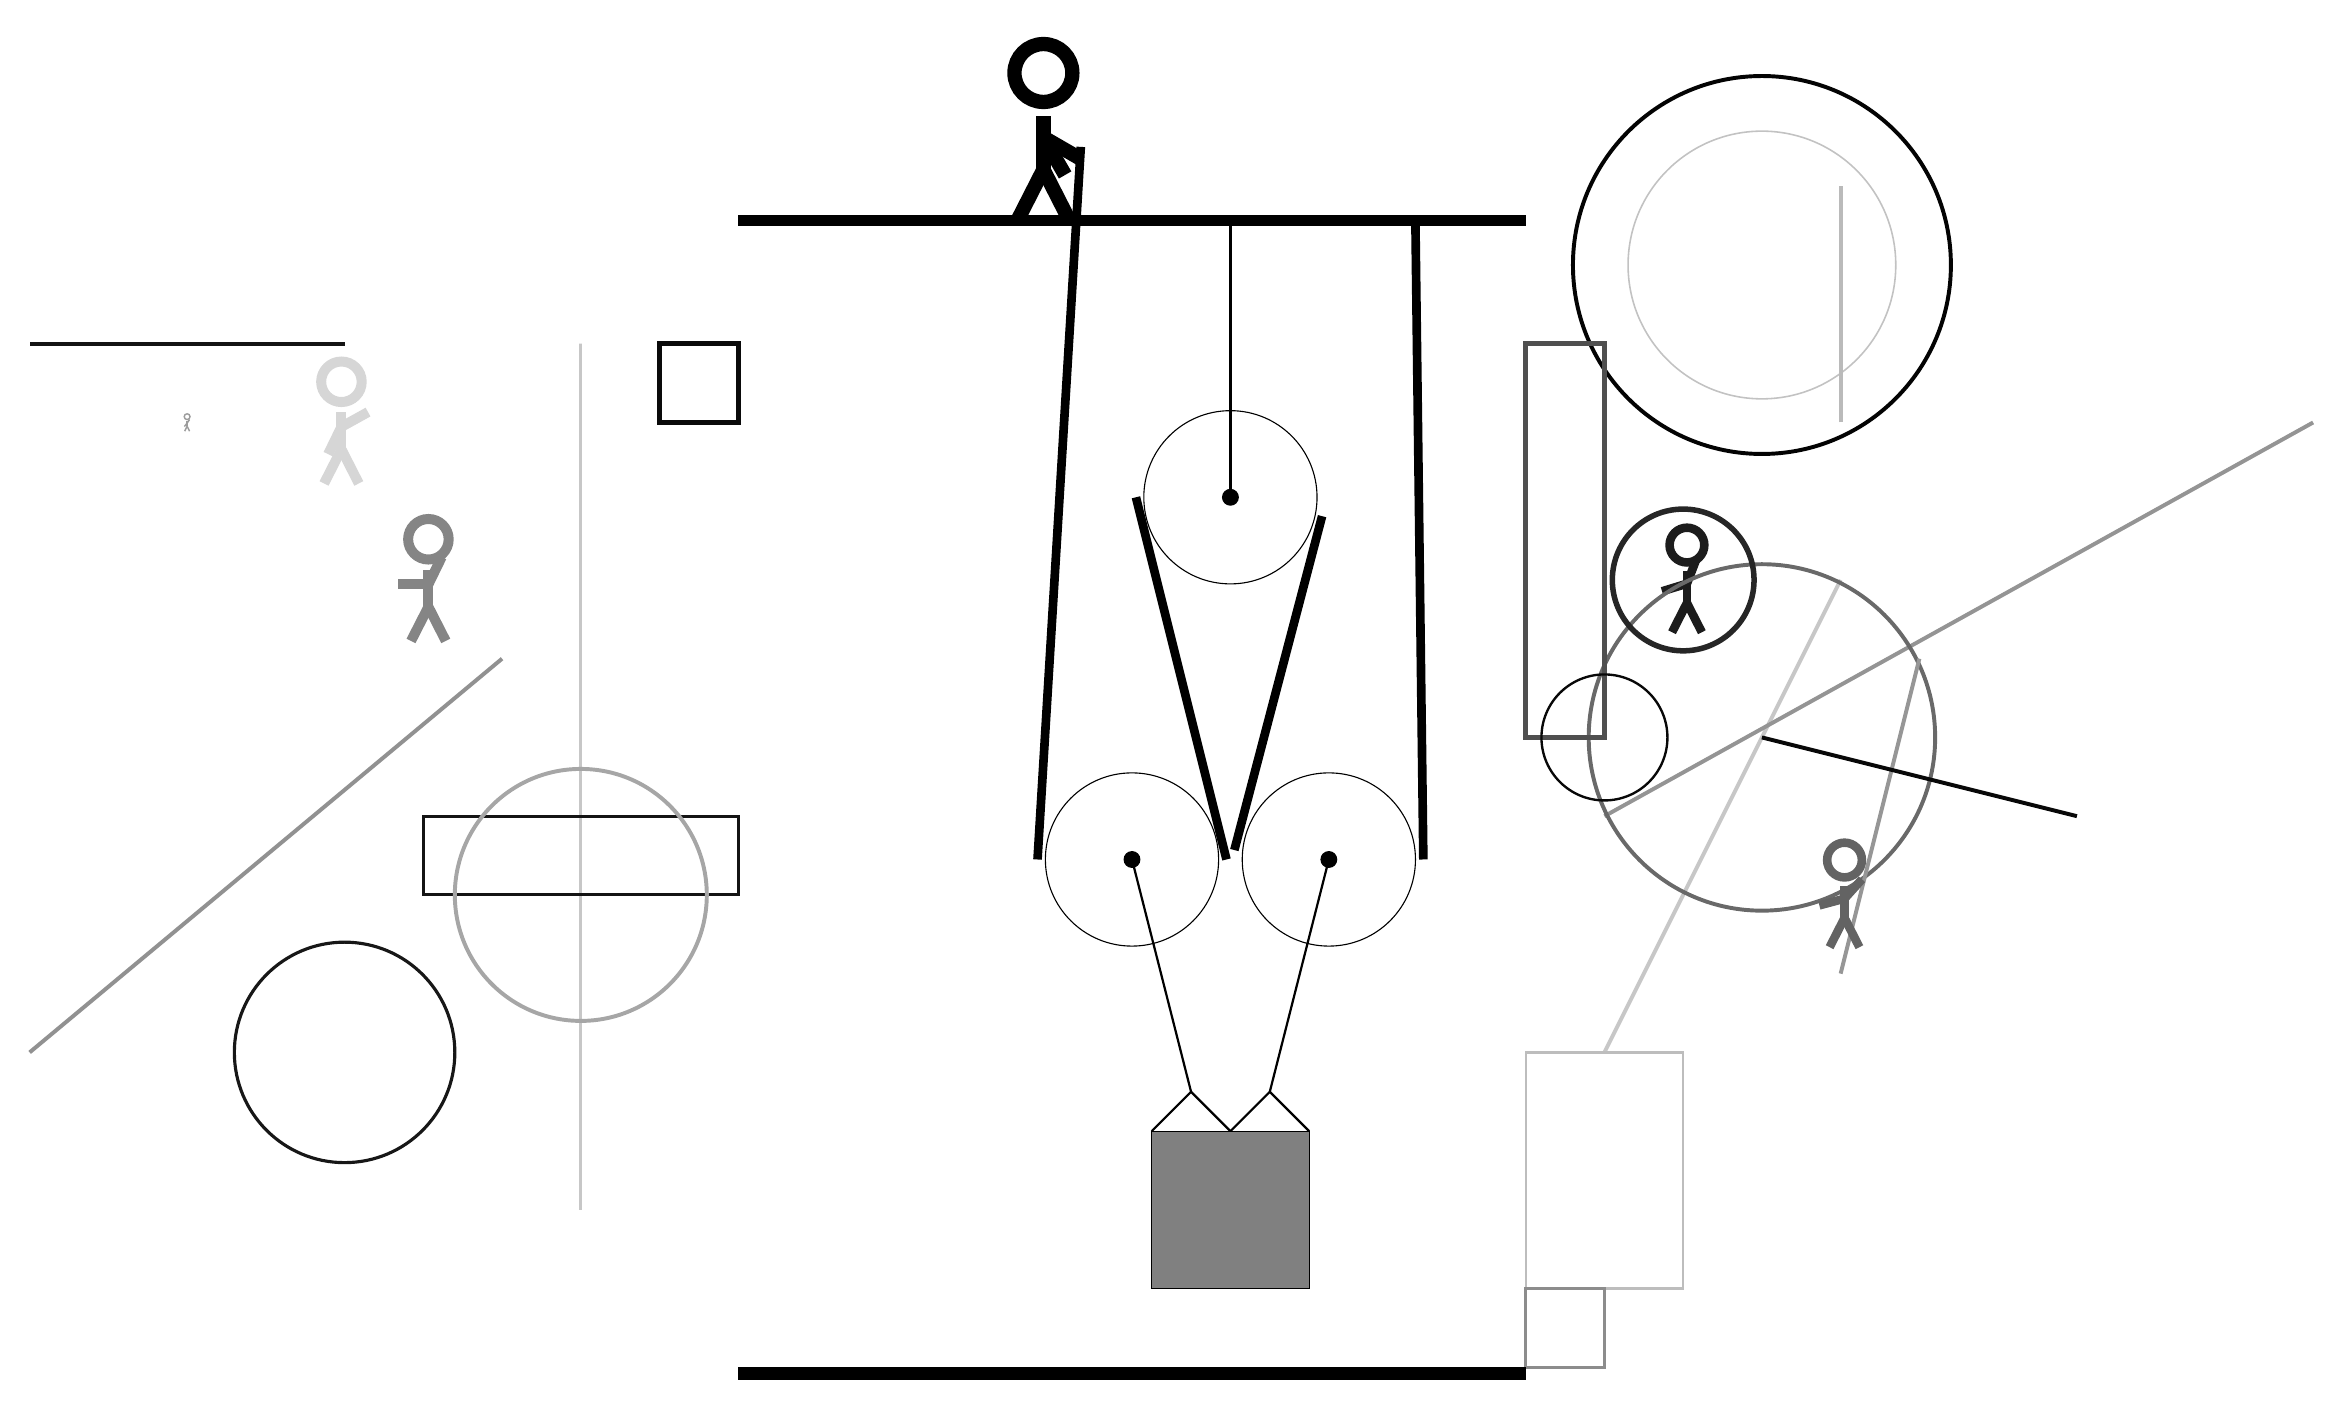
\begin{tikzpicture}
			%%%%% START %%%%%
			
			\draw[fill=black] (-4, 11.5) rectangle (6, 11.625);
			
			\draw[line width=0.5mm, color=black!22](10, 7) -- (7, 1);
			
			\draw[line width=0.3mm, color=black!26] (6, 1) rectangle (8, -2);
			\node[line width=0.2mm, color=black!39] at (-11, 9) {\Strichmaxerl[1][51][55]};
			\node[line width=0.3mm, color=black!48] at (-8, 7) {\Strichmaxerl[7][0][64]};
			\draw[line width=0.4mm, color=black!54] (-6, 3) rectangle (-6, 0);
			\draw [line width=0.4mm, color=black!91](-9, 1) circle (1.4);
			
			\draw[line width=0.7mm, color=black!96] (-5, 9) rectangle (-4, 10);
			\node[line width=0.3mm, color=black!89] at (8, 7) {\Strichmaxerl[6][17][69]};
			\draw[line width=0.5mm, color=black!42](7, 4) -- (16, 9);
			
			\draw [line width=0.5mm, color=black!59](9, 5) circle (2.2);
			\draw [line width=0.2mm, color=black!24](9, 11) circle (1.7);
			\draw[line width=0.5mm, color=black!92](-9, 10) -- (-13, 10);
			\draw[line width=0.5mm, color=black!41](10, 2) -- (11, 6);
			\draw[line width=0.4mm, color=black!45] (7, -3) rectangle (6, -2);
			\node[line width=0.4mm, color=black!16] at (-9, 9) {\Strichmaxerl[7][64][29]};
			\draw [line width=0.5mm, color=black!99](9, 11) circle (2.4);
			
			\draw[line width=0.7mm, color=black!69] (6, 10) rectangle (7, 5);
			\draw[line width=0.5mm, color=black!43](-7, 6) -- (-13, 1);
			\draw[line width=0.5mm, color=black!97](9, 5) -- (13, 4);
			
			\draw[line width=0.4mm, color=black!22] (-6, 10) rectangle (-6, -1);
			\draw[line width=0.4mm, color=black!92] (-4, 4) rectangle (-8, 3);
			
			\draw [line width=0.3mm, color=black!97](7, 5) circle (0.8);
			
			\draw [line width=0.7mm, color=black!85](8, 7) circle (0.9);
			\draw[line width=0.3mm, color=black!84] (7, 12) rectangle (7, 12);
			\node[line width=0.6mm, color=black!61] at (10, 3) {\Strichmaxerl[6][15][48]};
			\draw[line width=0.5mm, color=black!27](10, 9) -- (10, 12);
			
			\draw [line width=0.5mm, color=black!35](-6, 3) circle (1.6);
			
			\draw (1, 3.45) circle (1.1);
			\draw[fill=black] (1, 3.45) circle (0.1);
			
			\draw (2.25, 8.05) circle (1.1);
			\draw[fill=black] (2.25, 8.05) circle (0.1);
			\draw[thick] (2.25, 8.05) -- (2.25, 11.5);
			
			\draw (3.5, 3.45) circle (1.1);
			\draw[fill=black] (3.5, 3.45) circle (0.1);
			
			\draw[thick] (3.5, 3.45) -- (2.75, 0.5);
			\draw[thick] (1, 3.45) -- (1.75, 0.5);
			\draw[thick]  (1.25, 0) -- (1.75, 0.5) -- (2.25, 0);
			\draw[thick]  (2.25, 0) -- (2.75, 0.5) -- (3.25, 0);
			\draw[fill=black!50] (1.25, 0) rectangle (3.25, -2);
			
			\draw[line width=1.1mm] (0.35, 12.5) --  (-0.2, 3.45);
			\centerarc[line width=1.1mm](1, 3.45)(180:360:1.2000000000000002);
			\draw[line width=1.1mm] (2.2, 3.45) -- (1.05, 8.05);
			\centerarc[line width=1.1mm](2.25, 8.05)(-20:180:1.2000000000000002);
			\draw[line width=1.1mm](3.414, 7.81) -- (2.3, 3.57);
			\centerarc[line width=1.1mm](3.5, 3.45)(160:360:1.2000000000000002);
			\draw[line width=1.1mm](4.7, 3.45) -- (4.6, 11.5);
			
			\node at (-0.07, 12.7) {\Strichmaxerl[10][120][-30]};
			
			\draw[fill=black] (-4, -3) rectangle (6, -3.15);
			
			%%%%% END %%%%%
		\end{tikzpicture}
	\end{figure}	
\end{document}